\documentclass[border=10pt]{standalone}
\usepackage{tikz}
\usepackage{xcolor}
\usepackage{helvet}
\renewcommand{\familydefault}{\sfdefault}


% Define colors
\definecolor{masterblue}{RGB}{52, 152, 219}
\definecolor{slavegreen}{RGB}{46, 204, 113}
\definecolor{networkorange}{RGB}{230, 126, 34}

\begin{document}
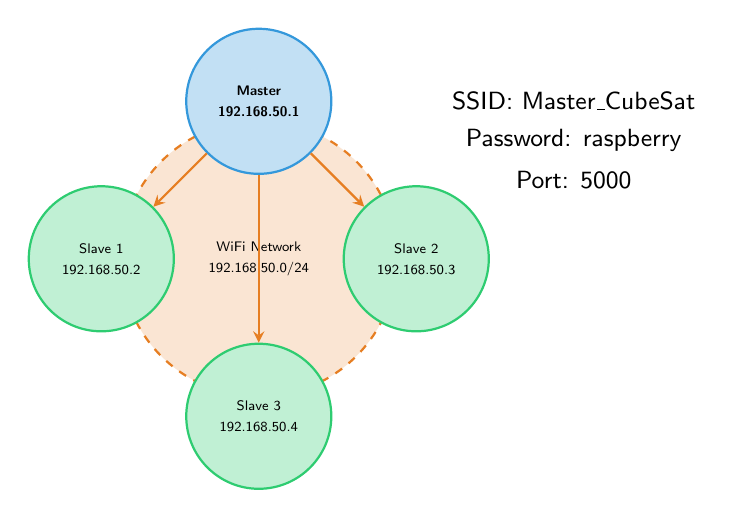
\begin{tikzpicture}[
    node distance=2cm,
    master/.style={circle, minimum size=1cm, fill=masterblue!30, draw=masterblue, thick, font=\tiny\bfseries},
    slave/.style={circle, minimum size=1cm, fill=slavegreen!30, draw=slavegreen, thick, font=\tiny},
    wifi/.style={circle, minimum size=3.5cm, fill=networkorange!20, draw=networkorange, thick, dashed, font=\tiny},
    connection/.style={->, thick, >=stealth, color=networkorange}
]

% WiFi network area
\node[wifi] (wifi) at (0,0) {\parbox{2cm}{\centering WiFi Network\\[0.3em] 192.168.50.0/24}};

% Master device
\node[master] (master) at (0,2) {\parbox{1.5cm}{\centering Master\\[0.3em] 192.168.50.1}};

% Slave devices
\node[slave] (slave1) at (-2,0) {\parbox{1.5cm}{\centering Slave 1\\[0.3em] 192.168.50.2}};
\node[slave] (slave2) at (2,0) {\parbox{1.5cm}{\centering Slave 2\\[0.3em] 192.168.50.3}};
\node[slave] (slave3) at (0,-2) {\parbox{1.5cm}{\centering Slave 3\\[0.3em] 192.168.50.4}};

% Connections
\draw[connection] (master) -- (slave1);
\draw[connection] (master) -- (slave2);
\draw[connection] (master) -- (slave3);

% Network info
\node[font=\small] at (4,2) {SSID: Master\_CubeSat};
\node[font=\small] at (4,1.5) {Password: raspberry};
\node[font=\small] at (4,1) {Port: 5000};

\end{tikzpicture}
\end{document}